\documentclass[11pt]{article}

\usepackage[margin=1in]{geometry}
\usepackage{amsmath,amssymb,mathtools,amsthm}
\usepackage{booktabs}
\usepackage{microtype}
\usepackage{graphicx}
\usepackage{tikz}
\usetikzlibrary{positioning,arrows.meta}
\usepackage[hidelinks]{hyperref}
\usepackage[nameinlink,capitalize]{cleveref}

\newtheorem{proposition}{Proposition}
\newtheorem{lemma}{Lemma}
\newtheorem{remark}{Remark}

\newcommand{\A}{\mathcal A}
\newcommand{\C}{\mathfrak C}
\newcommand{\F}{\mathcal F}
\newcommand{\eps}{\varepsilon}
\newcommand{\id}{\mathrm{id}}
\newcommand{\Tr}{\operatorname{Tr}}
\newcommand{\diam}{\operatorname{diam}}

\title{Finite-Data Non-Identification of Effective Quantum Coarse Dynamics}
\author{Tobias Croydon-McRae}
\date{Working manuscript --- 14 September 2026}

\begin{document}
\maketitle

\begin{abstract}
We study finite-data identification of a common effective update from a coarse quantum record.  In a fixed finite system ($N=8$), we consider the full class of source-independent, time-independent, whole-algebra completely positive trace-preserving (CPTP) maps on the proper coarse record $R2_{07}$, assessed by complete-source half-diamond error.  A rigorously certified map $\Phi_4$ fits four exposed transitions below tolerance $10^{-2}$.  That exact witness is frozen before two genuinely unseen transitions, selected by an outcome-blind schedule and provenance audit, are opened; it then fails both prospectively, with reviewed lower bounds $e_{F_1}(\Phi_4)\ge0.6246936110$ and $e_{F_2}(\Phi_4)\ge0.6217658418$.  After those failed predictions are added as constraints, the unchanged full physical map class remains feasible on all six transitions, with the hostile-reviewed bracket
\[
0.002306082156934015\ldots\le \eps_*^{(6)}\le
0.004582638648933954\ldots < 10^{-2}.
\]
Because the six-transition feasible set is a subset of the four-transition feasible set, the accepted six-transition witness is also four-transition feasible, while $\Phi_4$ is excluded by the two added constraints.  Thus the four-transition data do not uniquely identify a tolerance-feasible physical map: the finite model set contains at least two admissible maps with sharply different certified prospective errors.  We describe this as finite-data non-identification, or set-membership ambiguity.  The result is finite-system and finite-sample; it does not establish universal estimator failure, map-class misspecification, arbitrary-time autonomy, Markovianity or non-Markovianity, a semigroup, hidden-state necessity, or any continuum or gravitational claim.
\end{abstract}

\section{Introduction}
\label{sec:introduction}

If a restricted quantum record admits a common effective update on every transition observed so far, what has actually been learned about its future dynamics?

The existence of a physical map fitting a finite dataset is an important consistency statement, but it is not yet a predictive law or a point-identification result.  Finite observations can leave a non-singleton feasible model set, and representatives of that set can differ on directions or transitions not constrained by the observations.  Conversely, failure of one selected representative does not by itself show that the model class is misspecified.  These distinctions are standard in set-membership system identification, where finite data and uncertainty assumptions define a feasible set before any representative model is selected for prediction \cite{MilaneseNovara2004,MilaneseNovara2011}.  They also arise directly in incomplete quantum process tomography: incomplete process information can leave multiple channels compatible with the data, after which an additional selection principle may be used to choose a single estimator \cite{Ziman2008,TeoEtAl2011}.

This paper isolates the same logical distinction in a finite quantum coarse-dynamics setting where compatibility, selection of one witness, and later prospective testing can be certified separately.  We work with a fixed $N=8$ quantum system and a fixed proper coarse record denoted $R2_{07}$.  The admissible model class is deliberately broad: one physical, source-independent, time-independent, whole-algebra CPTP map on the full record algebra, with all central-sector transfers allowed.  The discrepancy on each transition is the half diamond norm of the difference between the next complete source-to-record channel and the channel obtained by applying the common map to the current source-to-record channel.

The reviewed finite sequence is as follows.  First, four already exposed transitions admit an explicit common map $\Phi_4$ with a rigorous error certificate below $10^{-2}$.  Second, that exact map is frozen, and two later transitions are chosen without access to their physical outcomes by an outcome-blind schedule plus an independent historical-exposure audit.  On those pristine transitions the frozen map fails by a large margin: independently reviewed lower bounds exceed $0.62$ on each transition.  Third, those failed predictions are added to the fitting constraints and the \emph{same full physical map class} is considered on the enlarged six-transition dataset.  A different explicit common map $\Phi_6$ fits all six transitions, and hostile review gives the rigorous minimax bracket
\begin{equation}
0.002306082156934015\ldots
\le \eps_*^{(6)}
\le 0.004582638648933954\ldots
<10^{-2}.
\label{eq:k6-bracket-intro}
\end{equation}
The failure is therefore a prospective failure of the selected four-transition witness, not a failure of the unchanged physical map class at six transitions.

The identification consequence is deterministic.  At tolerance $10^{-2}$, the four-transition feasible set contains at least two distinct physical maps with sharply different certified prospective errors.  The accepted map $\Phi_6$ lies in the six-transition feasible set and hence also in the four-transition feasible set, whereas $\Phi_4$ is excluded by the added prospective constraints.  The four finite observations therefore do not uniquely identify a tolerance-feasible physical map.  We use \emph{finite-data non-identification} and \emph{set-membership ambiguity} for this statement.  It does not imply that every possible estimator trained on four transitions must fail, that four transitions are information-theoretically insufficient under every prior or selection rule, or that the effective dynamics is fundamentally unknowable.

The distinction also blocks stronger dynamical readings.  A finite common-map fit is not automatically an autonomous law for arbitrary times, a quantum dynamical semigroup, a CP-divisible process, or a memoryless process.  Likewise, prospective failure of one witness does not prove non-Markovianity, hidden-state necessity, or missing state variables.  Operational approaches to multitime quantum processes make clear that such claims require richer interventions and temporal data \cite{PollockEtAl2018ProcessTensor,PollockEtAl2018Markov,WhiteEtAl2022}.

Our contribution is therefore a controlled finite case rather than a new general identification principle.  We (i) formulate the reviewed calculation as a finite common-channel identification problem; (ii) separate class compatibility, finite-set identification, witness selection, and prospective prediction; (iii) state the reviewed four-transition, prospective-failure, and six-transition certificates in one framework; (iv) use nested feasible sets to make the non-uniqueness deduction explicit; and (v) position this finite BCRD case relative to incomplete quantum process tomography, quantum system identification, finite CPTP interpolation, and classical set-membership identification.  The generic possibility of non-unique model sets under finite or incomplete data is established prior art; the contribution here is the custody-preserved, certified finite quantum instance.

The remainder of the paper is organized as follows.  \Cref{sec:framework} defines the identification problem and feasible-set semantics.  \Cref{sec:physical} specifies the finite record algebra and transition dataset.  \Cref{sec:results} presents the certified K=4 $\rightarrow$ prospective failure $\rightarrow$ K=6 sequence.  \Cref{sec:identification} develops the compatibility-versus-identification interpretation and future feasible-set diagnostics.  \Cref{sec:literature} situates the result within related identification and tomography literature, and \Cref{sec:discussion} states the limitations and nonclaims.

\section{Finite-data common-map identification}
\label{sec:framework}

\subsection{Transition channels and admissible maps}

Let $\A$ be a finite-dimensional $C^*$-algebra representing the retained coarse record, equipped with its physical trace $\tau$.  A complete source experiment at time $t$ is represented by a channel
\begin{equation}
\Lambda_t:M_2\longrightarrow \A,
\end{equation}
where the two-dimensional source is probed on all four matrix units, including its off-diagonal coherences.  For a sampled transition $j$ from $t_j$ to $t_j+\Delta$, write
\begin{equation}
\Lambda_j^{\mathrm{cur}}=\Lambda_{t_j},\qquad
\Lambda_j^{\mathrm{next}}=\Lambda_{t_j+\Delta}.
\end{equation}

The admissible class $\C$ consists of physical CPTP maps
\begin{equation}
\Phi:\A\to\A
\end{equation}
that are source-independent, time-independent and common to every transition in the dataset.  ``Physical'' refers to complete positivity together with preservation of the physical trace $\tau$ of the represented record algebra.  The map is defined on the whole algebra; computational support reductions are permitted only when accompanied by a CPTP extension/retraction argument establishing minimax equivalence to this whole-algebra problem.

For each transition define
\begin{equation}
e_j(\Phi)
=\frac12\left\|
\Lambda_j^{\mathrm{next}}
-\Phi\circ\Lambda_j^{\mathrm{cur}}
\right\|_\diamond .
\label{eq:error}
\end{equation}
The diamond norm retains the complete source-channel scope and the explicit factor $1/2$ is part of the frozen error convention.

For a finite transition dataset $D_K$ of cardinality $K$, define the minimax incompatibility
\begin{equation}
\eps_*^{(K)}
=\inf_{\Phi\in\C}\max_{j\in D_K}e_j(\Phi),
\label{eq:minimax}
\end{equation}
and, at tolerance $\eps\ge0$, the feasible set
\begin{equation}
\F_K(\eps)
=\left\{\Phi\in\C:
\max_{j\in D_K}e_j(\Phi)\le\eps
\right\}.
\label{eq:feasible-set}
\end{equation}
The compatibility question at tolerance $\eps$ is simply whether $\F_K(\eps)$ is nonempty.  It is logically distinct from whether the finite data identify a unique or predictively stable representative.

\subsection{Accumulating constraints}

The useful ordering variable is not a solver objective from one run but the minimax value of the full physical class under a genuinely nested data sequence.

\begin{lemma}[Nested feasible sets]
\label{lem:nesting}
If $D_K\subseteq D_{K+r}$ for $r>0$, with the same admissible class $\C$, error definition and tolerance, then
\begin{equation}
\F_{K+r}(\eps)\subseteq\F_K(\eps).
\label{eq:set-nesting}
\end{equation}
Consequently,
\begin{equation}
\eps_*^{(K)}\le\eps_*^{(K+r)}.
\label{eq:minimax-monotonicity}
\end{equation}
\end{lemma}

\begin{proof}
If $\Phi\in\F_{K+r}(\eps)$, then $e_j(\Phi)\le\eps$ for every $j\in D_{K+r}$.  Since $D_K\subseteq D_{K+r}$, the same inequalities hold for every $j\in D_K$, hence $\Phi\in\F_K(\eps)$.  For the minimax values, for every fixed $\Phi$,
\[
\max_{j\in D_K}e_j(\Phi)
\le
\max_{j\in D_{K+r}}e_j(\Phi).
\]
Taking the infimum over the same class $\C$ preserves the inequality.
\end{proof}

The lemma is elementary, but it prevents a recurrent interpretive error.  A particular witness may leave the feasible set when new constraints are added without the enlarged feasible set becoming empty.  Specifically,
\begin{equation}
\Phi_K\notin\F_{K+r}(\eps)
\qquad\not\Rightarrow\qquad
\F_{K+r}(\eps)=\varnothing.
\label{eq:witness-not-class}
\end{equation}
This distinction is the central logical point of the present example.

\subsection{Empty-feasible-set semantics}

A nonempty feasible set describes models compatible with the sampled data at the declared tolerance.  An empty feasible set has the opposite meaning: the entire model class is incompatible with those constraints at that tolerance.  Accordingly, geometric quantities such as $\diam\F_K(\eps)$ are left undefined (or explicitly marked inapplicable) when $\F_K(\eps)=\varnothing$.  We do not assign the empty set diameter zero and interpret this as perfect identification.

\subsection{Three questions}

We distinguish three levels throughout:

\paragraph{Class compatibility.}
Does there exist at least one $\Phi\in\C$ satisfying all observed transition constraints?  This is equivalent to $\F_K(\eps)\neq\varnothing$.

\paragraph{Witness identification or selection.}
How tightly do the finite observations constrain the map, and by what rule is a representative $\Phi_K$ selected?  A feasible point is not necessarily unique, minimax-optimal, statistically optimal, or stable outside the constrained domain.

\paragraph{Prospective prediction.}
Does a previously frozen $\Phi_K$ accurately reproduce genuinely unseen transitions without refitting?  This is an out-of-sample test of that fixed witness, not an all-map existence test unless an additional universal certificate is supplied.

No implication among these questions should be assumed beyond what is proved from the data and class definitions.

\section{Physical finite-system setting}
\label{sec:physical}

\subsection{\texorpdfstring{The $N=8$ proper record $R2_{07}$}{The N=8 proper record R2-07}}

We specialize the framework to one frozen finite model: $N=8$, no-cursor Candidate E, isotropic coupling $J=1$, and proper coarse record $R2_{07}$.  Five register qubits $R_1,\ldots,R_5$ are retained, with the complete source qubit carried by $R_5$.  The matter record is generated by
\begin{equation}
\operatorname{alg}^*(D_{12},D_{34},D_{56},D_{67}).
\end{equation}
Its reviewed central decomposition is most transparently labeled by $(j_{12},j_{34},2j_{567})$:
\begin{center}
\begin{tabular}{c c c c c c}
\toprule
$a$ & $(j_{12},j_{34},2j_{567})$ & $n_a$ & $m_a$ & $d_a=32n_a$ & concrete width $d_am_a$\\
\midrule
0 & $(0,0,1)$ & 2 & 1 & 64 & 64\\
1 & $(0,1,1)$ & 2 & 1 & 64 & 64\\
2 & $(0,1,3)$ & 1 & 1 & 32 & 32\\
3 & $(1,0,1)$ & 2 & 1 & 64 & 64\\
4 & $(1,0,3)$ & 1 & 1 & 32 & 32\\
5 & $(1,1,1)$ & 2 & 2 & 64 & 128\\
6 & $(1,1,3)$ & 1 & 2 & 32 & 64\\
\bottomrule
\end{tabular}
\end{center}
Thus the abstract record algebra is
\begin{equation}
\A_{R2_{07}}
\cong \bigoplus_{a=0}^{6}M_{d_a},
\qquad
(d_a)=(64,64,32,64,32,64,32),
\label{eq:record-algebra}
\end{equation}
with concrete representation $x_a\mapsto x_a\otimes I_{m_a}$ and multiplicity vector
\begin{equation}
(m_a)=(1,1,1,1,1,2,2).
\end{equation}
The physical trace is therefore
\begin{equation}
\tau(x)=\sum_{a=0}^6 m_a\Tr(x_a),
\label{eq:physical-trace}
\end{equation}
not the unweighted abstract direct-sum trace.  The reviewed density-coordinate map $y_a=m_ax_a$ is a complete order/trace isomorphism to ordinary sum-trace coordinates, represented concretely by $y_a\mapsto y_a\otimes I_{m_a}/m_a$.

Every linear map on the direct-sum algebra decomposes into central components $\Phi_{ba}:M_{d_a}\to M_{d_b}$.  The full admissible class allows all $7\times7=49$ transfers.  Complete positivity is equivalent to positivity of every component Choi matrix, together with the physical weighted trace-preservation conditions.  No block-diagonal-in-center restriction is imposed.

\subsection{Complete source channels}

For a source density operator $\rho\in M_2$, the frozen microscopic evolution and record expectation define
\begin{equation}
\Lambda_t(\rho)
=E_{\mathrm{rec}}
\bigl(e^{-itH}X\rho X^\dagger e^{itH}\bigr),
\label{eq:source-channel}
\end{equation}
where $H$, the source embedding $X$, and $E_{\mathrm{rec}}$ are fixed by the physical model.  All four source matrix units $E_{00},E_{01},E_{10},E_{11}$ are retained.  Consequently, the error in \cref{eq:error} is a complete source-channel error rather than a finite state-mesh discrepancy.

\subsection{The six opened transitions}

The scientific dataset used in this paper is exactly
\begin{equation}
D_6=\{\mathrm{TRAIN0},\mathrm{TRAIN1},H_1,H_2,F_1,F_2\}.
\end{equation}
The canonical K=6 custody packet binds 11 already-authorized floating-point endpoint values.  The exact renderings used by the reviewed evaluator are listed in \cref{tab:transitions}.  No additional time is opened or evaluated in this writing lane.

\begin{table}[ht]
\centering
\caption{Frozen transition dataset.  The TRAIN0/TRAIN1 shared endpoint is the historically banked binary64 value $0.9323881824729999$; the independently typed decimal $0.932388182473$ is one ULP away.  $F_1$ and $F_2$ were selected prospectively by an outcome-blind schedule after an independent historical-exposure audit established the exposure frontier.}
\label{tab:transitions}
\begin{tabular}{lrrl}
\toprule
transition & current time & next time & role\\
\midrule
TRAIN0 & 0.832388182473 & 0.9323881824729999 & original training\\
TRAIN1 & 0.9323881824729999 & 1.032388182473 & original training\\
$H_1$ & 1.232388182473 & 1.332388182473 & exposed K=4 constraint\\
$H_2$ & 1.382388182473 & 1.482388182473 & exposed K=4 constraint\\
$F_1$ & 24.232388182473 & 24.332388182473 & pristine prospective\\
$F_2$ & 24.532388182473 & 24.632388182473 & pristine prospective\\
\bottomrule
\end{tabular}
\end{table}

The prospective schedule was not chosen after viewing $F_1$ or $F_2$.  An outcome-blind rule was frozen first; a separate provenance audit established $t_{\rm exposed,max}=24$ and mechanically selected the two-transition block.  Both transitions were opened as one atomic packet before either was classified.  This custody matters scientifically because the later failure of $\Phi_4$ is used as genuine prospective evidence rather than merely another post-hoc residual.

\section{Certified finite-data phenomenon}
\label{sec:results}

\subsection{Four-transition common-map compatibility}

Let
\begin{equation}
D_4=\{\mathrm{TRAIN0},\mathrm{TRAIN1},H_1,H_2\}.
\end{equation}
A frozen whole-algebra physical CPTP map, denoted $\Phi_4$, was constructed for this dataset and then independently hostile-reviewed.  Its immutable artifact digest is
\begin{center}
\texttt{48abd5f52812ef7503cfdde92fe630b99ded9c10c4ef35d2c4edc8d934028125}.
\end{center}
The artifact contains all 49 central transfers and 5184 Kraus operators, with exact structural complete positivity and physical trace preservation after the frozen completion.  An independent exact certificate gives
\begin{equation}
\max_{j\in D_4}e_j(\Phi_4)
\le 0.006670414972746646\ldots <10^{-2}.
\label{eq:k4-upper}
\end{equation}
A reduction-free hostile ambient-dual certificate also gives the universal lower
\begin{equation}
\eps_*^{(4)}\ge 0.00028544924736174324\ldots .
\end{equation}
Hence the four-transition class is nonempty at the declared tolerance:
\begin{equation}
\Phi_4\in\F_4(10^{-2}).
\label{eq:phi4-feasible}
\end{equation}
This is a finite compatibility statement only.  At this stage $\Phi_4$ had no authority as an arbitrary-time law or as a prospectively validated predictor.

\subsection{Prospective failure of the frozen witness}

The exact artifact in \cref{eq:phi4-feasible} was frozen before the $F_1,F_2$ physical values were opened.  The outcome-blind schedule/provenance chain described in \cref{sec:physical} then selected the two pristine transitions.  On those transitions, simple rigorous lower certificates for the complete-source half-diamond error give
\begin{align}
e_{F_1}(\Phi_4)&\ge0.6246936110454476,\\
e_{F_2}(\Phi_4)&\ge0.6217658417777687.
\label{eq:phi4-forward-failure}
\end{align}
Both exceed the tolerance $10^{-2}$ by more than sixty-fold.  A fresh reviewer-owned full recomputation was subsequently executed and agreed with the banked result.  Therefore
\begin{equation}
\Phi_4\notin\F_6(10^{-2}).
\label{eq:phi4-not-f6}
\end{equation}
Crucially, \cref{eq:phi4-not-f6} says nothing by itself about whether $\F_6(10^{-2})$ is empty.

\begin{figure}[ht]
\centering
% Schematic custody/inference figure. Vertical layout prevents clipping and does not imply uniqueness.
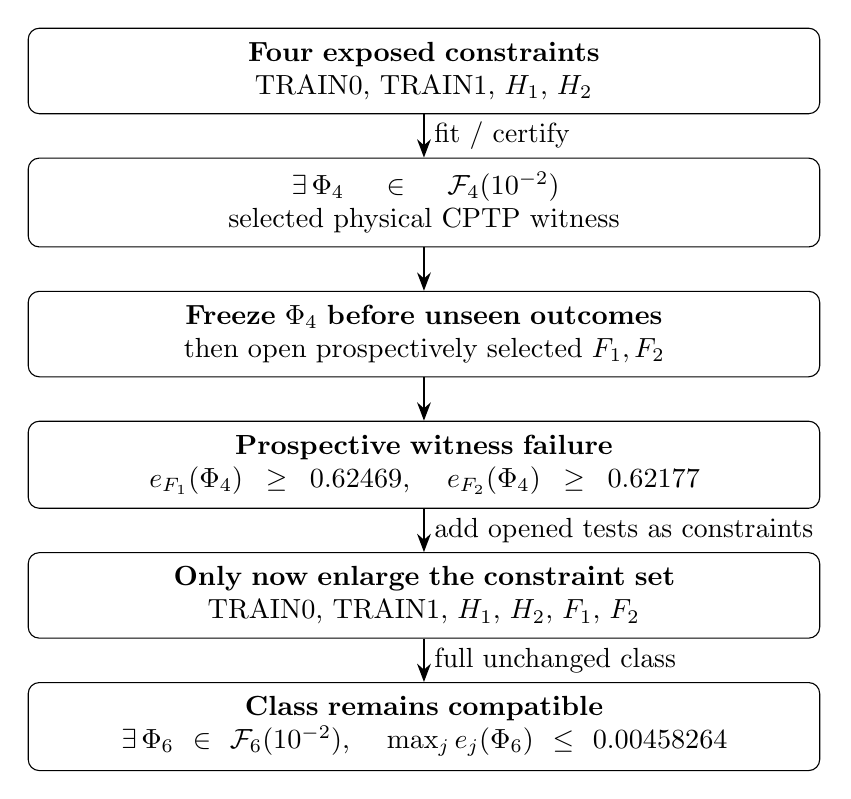
\begin{tikzpicture}[
  node distance=0.55cm,
  >=Stealth,
  box/.style={draw,rounded corners,align=center,text width=0.80\linewidth,inner sep=5pt},
  arrow/.style={->,thick}
]
\node[box] (d4) {\textbf{Four exposed constraints}\\TRAIN0, TRAIN1, $H_1$, $H_2$};
\node[box,below=of d4] (p4) {$\exists\,\Phi_4\in\F_4(10^{-2})$\\selected physical CPTP witness};
\node[box,below=of p4] (freeze) {\textbf{Freeze $\Phi_4$ before unseen outcomes}\\then open prospectively selected $F_1,F_2$};
\node[box,below=of freeze] (fail) {\textbf{Prospective witness failure}\\
$e_{F_1}(\Phi_4)\ge 0.62469$, \quad
$e_{F_2}(\Phi_4)\ge 0.62177$};
\node[box,below=of fail] (d6) {\textbf{Only now enlarge the constraint set}\\TRAIN0, TRAIN1, $H_1$, $H_2$, $F_1$, $F_2$};
\node[box,below=of d6] (p6) {\textbf{Class remains compatible}\\
$\exists\,\Phi_6\in\F_6(10^{-2})$, \quad
$\max_j e_j(\Phi_6)\le0.00458264$};

\draw[arrow] (d4) -- node[right]{fit / certify} (p4);
\draw[arrow] (p4) -- (freeze);
\draw[arrow] (freeze) -- (fail);
\draw[arrow] (fail) -- node[right]{add opened tests as constraints} (d6);
\draw[arrow] (d6) -- node[right]{full unchanged class} (p6);
\end{tikzpicture}

\caption{The custody and inference sequence.  The four-transition data first certify one feasible witness $\Phi_4$, which is frozen before the unseen $F_1,F_2$ tests.  Failure of that fixed witness is then established prospectively.  Only after the new transitions are opened are they added to the constraint set, where a separate six-transition existence calculation certifies a witness $\Phi_6$.  The diagram does not imply that $\Phi_4$ was unique at K=4 or that $\Phi_6$ was obtained before $F_1,F_2$ were opened.}
\label{fig:fit-prediction}
\end{figure}

\subsection{Six-transition class compatibility after enlargement}

After $F_1$ and $F_2$ had been opened and their failure for $\Phi_4$ established, they were added as constraints rather than used to alter the physical model class.  The six-transition problem therefore uses exactly the same $\C$ as the K=4 problem.  An explicit whole-algebra map $\Phi_6$ was certified with artifact digest
\begin{center}
\texttt{c674e471c6bbad2e3376e53315d8e1e5cb83dbbb85f4120c7b5b8602b78f7e0a}.
\end{center}
Fresh hostile review independently reconstructed the complete-source residuals and certified the per-transition upper bounds in \cref{tab:k6-uppers}.

\begin{table}[ht]
\centering
\caption{Hostile-reviewed rigorous upper certificates for the accepted six-transition witness $\Phi_6$.}
\label{tab:k6-uppers}
\begin{tabular}{lr}
\toprule
transition & rigorous upper on $e_j(\Phi_6)$\\
\midrule
TRAIN0 & 0.0017360413721420206\\
TRAIN1 & 0.0017902995810885707\\
$H_1$ & 0.0017010819506354795\\
$H_2$ & 0.0022602480754981130\\
$F_1$ & 0.0045826386489339540\\
$F_2$ & 0.0044800043819739690\\
\bottomrule
\end{tabular}
\end{table}

The worst certified transition is $F_1$, so
\begin{equation}
\max_{j\in D_6}e_j(\Phi_6)
\le0.004582638648933954\ldots<10^{-2}.
\label{eq:k6-upper}
\end{equation}
A universal lower certificate, obtained from the subset TRAIN0+$F_1$+$F_2$ and lifted to the ambient whole-algebra problem, survived independent review at
\begin{equation}
\eps_*^{(6)}\ge0.002306082156934015\ldots .
\label{eq:k6-lower}
\end{equation}
Combining \cref{eq:k6-upper,eq:k6-lower} yields
\begin{equation}
\boxed{
0.002306082156934015\ldots
\le\eps_*^{(6)}
\le0.004582638648933954\ldots
<10^{-2}}
\label{eq:k6-bracket}
\end{equation}
and hence
\begin{equation}
\F_6(10^{-2})\neq\varnothing.
\label{eq:f6-nonempty}
\end{equation}

\begin{figure}[ht]
\centering
% Abstract set-membership schematic; boxes carry no metric/geometric meaning.
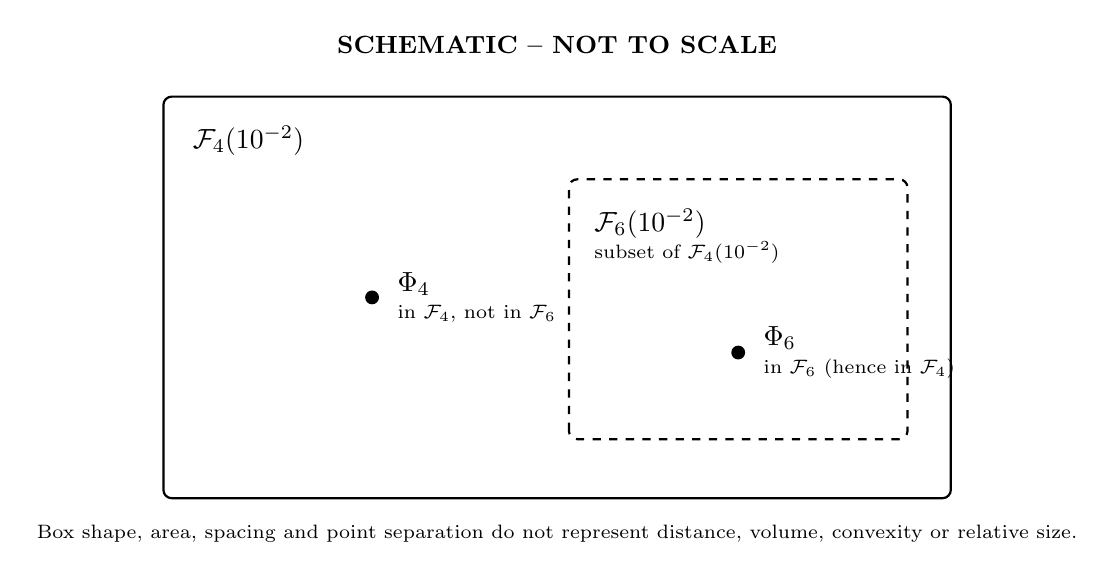
\begin{tikzpicture}[x=1cm,y=1cm]
  \node[font=\small\bfseries] at (0,3.35) {SCHEMATIC -- NOT TO SCALE};
  \draw[thick,rounded corners=3pt] (-5,-2.4) rectangle (5,2.7);
  \node[anchor=north west] at (-4.75,2.45) {$\mathcal F_4(10^{-2})$};

  \draw[thick,dashed,rounded corners=3pt] (0.15,-1.65) rectangle (4.45,1.65);
  \node[anchor=north west,align=left] at (0.35,1.40)
    {$\mathcal F_6(10^{-2})$\\[-2pt]\scriptsize subset of $\mathcal F_4(10^{-2})$};

  \fill (-2.35,0.15) circle (2.5pt);
  \node[anchor=west,align=left] at (-2.15,0.15)
    {$\Phi_4$\\[-2pt]\scriptsize in $\mathcal F_4$, not in $\mathcal F_6$};

  \fill (2.30,-0.55) circle (2.5pt);
  \node[anchor=west,align=left] at (2.50,-0.55)
    {$\Phi_6$\\[-2pt]\scriptsize in $\mathcal F_6$ (hence in $\mathcal F_4$)};

  \node[align=center,font=\scriptsize] at (0,-2.85)
    {Box shape, area, spacing and point separation do not represent distance, volume, convexity or relative size.};
\end{tikzpicture}

\caption{Schematic set-membership relation, not to scale.  Only $\F_6(10^{-2})\subseteq\F_4(10^{-2})$ and the marked membership/exclusion statements are asserted.  Box shape, area, spacing and point separation carry no geometric, metric, volume or convexity claim.}
\label{fig:nested-sets}
\end{figure}

\subsection{Central certified proposition}

\begin{proposition}[Frozen finite-system phenomenon]
\label{prop:central}
For the frozen $N=8$, $R2_{07}$ transition family and the full physical class $\C$ at tolerance $10^{-2}$:
\begin{enumerate}
\item $\Phi_4\in\F_4(10^{-2})$;
\item $\Phi_4\notin\F_6(10^{-2})$ because it fails both genuinely unseen $F_1,F_2$ transitions by the reviewed bounds in \cref{eq:phi4-forward-failure};
\item $\F_6(10^{-2})\neq\varnothing$, with the minimax bracket in \cref{eq:k6-bracket}.
\end{enumerate}
Therefore prospective failure of the frozen four-transition witness does not imply failure of six-transition common-map compatibility.
\end{proposition}

\begin{proof}
Item 1 follows from the certified bound \cref{eq:k4-upper}.  Item 2 follows because each lower bound in \cref{eq:phi4-forward-failure} is larger than $10^{-2}$.  Item 3 follows constructively from the certified whole-algebra witness $\Phi_6$ and \cref{eq:k6-upper}; the universal lower in \cref{eq:k6-lower} supplies the stated minimax bracket.  The final implication is immediate: one point $\Phi_4$ leaves the nested feasible set, while another point $\Phi_6$ remains.
\end{proof}

An additional deterministic consequence supplies the identification statement.  Since $D_4\subset D_6$, \cref{lem:nesting} gives $\F_6(10^{-2})\subseteq\F_4(10^{-2})$.  Therefore $\Phi_6\in\F_4(10^{-2})$ as well.  Together with $\Phi_4\in\F_4(10^{-2})$ and $\Phi_4\notin\F_6(10^{-2})$, this proves $\Phi_4\neq\Phi_6$ and shows that the K=4 tolerance-feasible set contains at least two distinct physical maps with sharply different certified prospective errors.  This is finite-data non-identification at the declared tolerance; it is not a theorem that every possible K=4 estimator has poor future risk.

\section{Compatibility versus identification}
\label{sec:identification}

\subsection{What the four-transition fit identified}

The K=4 result establishes a nonempty feasible subset of the physical map class, not a unique law.  At tolerance $10^{-2}$, both $\Phi_4$ and $\Phi_6$ satisfy the first four constraints, yet only $\Phi_6$ satisfies the added $F_1,F_2$ constraints.  The finite K=4 observations therefore do not collapse the tolerance-feasible model set to a singleton, and unconstrained map freedom matters on the later certified transitions.

We call this \emph{finite-data non-identification}, equivalently a \emph{set-membership ambiguity} at the declared tolerance.  The statement is relative to the chosen physical class, observation family and tolerance: the data admit distinguishable physical maps whose certified errors differ sharply on later admissible transitions.  It should not be read as a claim that the microscopic model itself is ambiguous, that every K=4 selection rule must fail, or that no alternative experiment could identify an effective map more tightly.

Nor is ``overfitting'' the right primary technical term.  Classical overfitting normally invokes a specified estimator, a stochastic data-generating model, model complexity and an out-of-sample risk distribution.  Here the load-bearing statements are deterministic: membership in a finite feasible set, custody of a frozen witness, a prospective failure certificate, and survival of the full feasible class after the constraints are enlarged.  ``Prospective failure of the frozen selected witness'' is therefore the precise event; finite-data non-identification is the set-level interpretation.

\subsection{Feasible-set motion as the natural next diagnostic}

The certified sequence motivates, but does not yet numerically determine, the geometry of $\F_K(\eps)$.  For a metric $d$ on physical maps one might study
\begin{equation}
D_K^d(\eps)=\sup_{\Phi,\Psi\in\F_K(\eps)}d(\Phi,\Psi),
\label{eq:diameter-diagnostic}
\end{equation}
together with directed displacement or Hausdorff-like quantities between nested feasible sets.  Because $\F_{K+r}\subseteq\F_K$, ordinary symmetric Hausdorff distance reduces to the maximum distance of a point in the larger set $\F_K$ from the smaller surviving set $\F_{K+r}$, provided the sets are nonempty and the metric topology is specified.

Two metric choices should be kept distinct.  A \emph{whole-algebra map metric} probes differences on all directions in $\A_{R2_{07}}$, including directions not reached by the finite source family at the sampled times.  A \emph{reachable-domain metric} restricts attention to the physically source-accessible/channel-reachable subset.  A map pair can be far apart globally while agreeing closely on the observed domain, so these diagnostics answer different identification questions.

One may also define a canonical selector $S_K$---for example a regularized minimax center fixed before seeing later data---and inspect
\begin{equation}
d\bigl(S_K(D_K),S_{K+r}(D_{K+r})\bigr).
\end{equation}
No such selector is analyzed here.  In particular, the historical $\Phi_4$ and $\Phi_6$ should not be promoted into a general canonical-estimator theorem merely because they provide a concrete example of feasible-set contraction.

\subsection{Compatibility obstruction versus identification contraction}

The monotone scalar $\eps_*^{(K)}$ and the structure of $\F_K(\eps)$ encode different information.  The former asks how close the best common map can come to the accumulated constraints.  The latter asks how much freedom remains among maps that meet a chosen tolerance.  It is possible for $\eps_*^{(K)}$ to remain below tolerance while the feasible set contracts substantially, or for a non-singleton feasible set to persist until a new constraint makes it empty.

The present K=4-to-K=6 sequence establishes only the finite set-membership fact needed here.  The K=6 optimum is still below $0.01$, while one previously valid point is excluded by the new constraints.  Future nested-K work could quantify feasible-set motion, but no diameter, Hausdorff distance, volume or canonical-selector stability value is computed in this paper.

\subsection{Empty sets are incompatibility, not identification}

If a later nested dataset yields $\F_K(\eps)=\varnothing$, the correct conclusion is model-class incompatibility at that tolerance.  Geometric identification measures that presuppose a nonempty feasible set must then be marked undefined.  Assigning an empty-set diameter of zero and calling it ``perfect identification'' would reverse the scientific meaning of the result.

\section{Relation to process tomography and system identification}
\label{sec:literature}

\subsection{Incomplete and finite quantum-process identification}

Quantum process tomography asks how an unknown channel can be reconstructed from controlled preparations and measurements.  Foundational prescriptions show how informationally complete experiments can characterize an arbitrary open-system process \cite{ChuangNielsen1997,PoyatosCiracZoller1997}; later work analyzes resource costs and structured reductions such as compressive process tomography \cite{MohseniRezakhaniLidar2008,ShabaniEtAl2011}.  Gate-set tomography addresses a related self-consistency problem in which state preparation, gates and measurement cannot be treated as independently calibrated objects \cite{BlumeKohoutEtAl2017}.

Directly relevant here is the literature on \emph{incomplete} quantum process data.  Ziman studies process estimation when the available information does not determine a unique channel and uses a maximum-entropy principle to select an estimate from the remaining compatible possibilities \cite{Ziman2008}.  Teo \emph{et al.} likewise treat incomplete process-tomography data for which the observations do not uniquely specify the process, introducing an additional maximum-likelihood/maximum-entropy selection procedure \cite{TeoEtAl2011}.  These works make the general quantum identification point explicit: incomplete process information can define a non-singleton compatible set, while a unique reported estimator requires an additional selection rule.

Our setting differs in both data source and error model.  The microscopic evolution is known and the finite source-to-record channels are computed and certified; the uncertainty is which effective \emph{common} CPTP map is identified by a finite set of deterministic complete-source transition constraints.  The finite constraints are not an informationally complete tomography experiment for $\Phi$ on the whole record algebra.  Accordingly, non-uniqueness of the compatible quantum process set is not claimed as novel.

Finite CPTP interpolation provides a neighboring mathematical perspective.  Alberti--Uhlmann-type questions ask whether a CPTP map can send prescribed input states to prescribed output states; modern refinements give sharp conditions in specialized cases \cite{ChakrabortyEtAl2020}.  The BCRD optimization can be viewed as an approximate, complete-channel, repeated-common-map interpolation problem with a physically weighted direct-sum algebra.  Again, nothing in the present result claims novelty for the generic fact that finite interpolation constraints may admit multiple CPTP maps.

\subsection{System identification and set membership}

Quantum system identification studies what features of an underlying dynamical system are estimable from available input-output experiments \cite{BurgarthYuasa2012}.  Classical set-membership identification supplies the closest terminology for the present deterministic inference: finite or uncertainty-bounded data define a feasible model set, and identification and prediction are distinct questions posed over that set \cite{MilaneseNovara2004,MilaneseNovara2011}.  In this language, $\F_K(\eps)$ is a finite quantum feasible-model set and the prospective $F_1,F_2$ experiment tests one previously selected point from that set.

The analogy has limits.  Our tolerance is a deterministic complete-channel error threshold rather than a probabilistic confidence region; the admissible set is constrained by complete positivity and physical trace preservation; and the transition channels are derived from a fixed finite quantum model rather than noisy laboratory samples in the present study.  These differences are why we retain the precise CPTP/diamond-norm formulation rather than translating the result wholesale into classical identification terminology.

\subsection{Why the result is not a Markovianity test}

A one-step map that fits finitely many transitions is much weaker than a multitime Markov property.  Process-tensor approaches characterize a quantum process operationally through interventions across multiple times and make memory statements at that level \cite{PollockEtAl2018ProcessTensor,PollockEtAl2018Markov}.  Non-Markovian process tomography similarly requires multitime information beyond a list of compatible one-step transitions \cite{WhiteEtAl2022}.  Therefore neither the K=6 compatibility result nor the prospective failure of $\Phi_4$ is a valid standalone test of Markovianity.

The same caution applies to semigroup language.  We do not establish $\Phi_{t+s}=\Phi_t\Phi_s$, CP-divisibility, a Lindblad generator, or even that the same map describes every interval of length $\Delta$ outside the six sampled transitions.  ``Common-map compatibility'' in this paper always means compatibility on the explicitly listed finite transition family.

\subsection{Contribution relative to prior art}

The general framework is known: finite or incomplete data can leave a model set non-unique, including in quantum process estimation.  The BCRD-specific contribution is the reviewed finite conjunction
\[
\begin{gathered}
\text{K=4 compatibility}
\to
\text{exact witness frozen}
\to
\text{pristine prospective failure}
\\
\to
\text{unchanged-class K=6 compatibility}.
\end{gathered}
\]
with explicit physical map artifacts, rigorous prospective lower certificates, a hostile-reviewed K=6 lower/upper minimax bracket, and custody that fixes when the later transition outcomes became available.

We therefore present the result as a controlled certified case study.  We make no priority claim for finite-data non-identification, set-membership ambiguity, incomplete process tomography, prospective validation, or the elementary nesting lemma.  The evidential architecture is documented so that the finite case can be audited, not advertised as a new general theorem.

\section{Discussion and limitations}
\label{sec:discussion}

\subsection{What has been learned}

The main scientific lesson is narrower than ``the effective dynamics failed'' and more informative than ``one fit was bad.''  At K=4, the physical common-map class is compatible with the data and contains at least two distinct tolerance-feasible maps.  The historically selected $\Phi_4$ is one such map.  When subjected without refitting to genuinely unseen transitions, it fails strongly.  Yet those same new transitions do not invalidate the map class: a second physical map fits all six, with a hostile-reviewed minimax optimum bounded strictly below the same tolerance.

The clean interpretation is therefore a separation of \emph{compatibility}, \emph{finite-data identification}, and \emph{prospective prediction}.  The four finite constraints do not uniquely identify a tolerance-feasible map and do not force the selected witness's behavior on the later transitions.  Adding the later constraints contracts the feasible set and excludes $\Phi_4$, but does not make the set empty.

This distinction also clarifies why a negative prospective test remains informative when the class subsequently survives.  The prospective failure rules out a particular frozen candidate as an accurate predictor for $F_1,F_2$ and demonstrates that its earlier fit did not by itself warrant that extrapolation.  The six-transition compatibility result then localizes the conclusion: at this finite stage, fitting the newly opened transitions does not require enlarging the physical record or abandoning the full common-CPTP class.  It does not show that the class will survive further constraints.

\subsection{Finite scope}

The result concerns exactly one finite system ($N=8$), one proper coarse record ($R2_{07}$), one complete source family, six sampled transitions and tolerance $10^{-2}$.  It does not establish persistence as more transitions are accumulated.  In particular, $\eps_*^{(K)}$ is monotone nondecreasing under nested constraints, so a later K may still cross the tolerance.  The present paper stops at the reviewed K=6 cutoff.

Likewise, no cross-$N$ statement follows.  Even if the same record construction can be defined at other system sizes, compatibility, feasible-set structure and prospective behavior must be established independently there.  No large-$N$ or continuum conclusion is drawn.

\subsection{No autonomy or memory claim}

Finite sampled common-map compatibility does not imply an arbitrary-time autonomous effective law.  The six-transition result says only that a single physical map can jointly approximate those six one-step channels.

Prospective failure of $\Phi_4$ also does not establish memory.  A memory interpretation would require an operational multitime test or an independently justified state-augmentation theorem.  It is logically possible for a different one-step map on the same record to fit the enlarged finite set---indeed that is what the K=6 certificate proves.  Hidden-state necessity, minimal augmentation and Markov order therefore remain open.

\subsection{Computational reductions and certificate hygiene}

The accepted six-transition result is a statement about the whole-algebra class.  The P/Q support construction used to make the optimization tractable is described only as exact minimax-equivalent through CPTP extension/retraction.  It is not a literal equality between the reduced and global map sets.  The certified witness itself is explicitly completed to a whole-algebra physical CPTP map.

The review chain also identified pseudo-exact arithmetic in older auxiliary spectral routines based on object arrays that still contained binary floating-point values.  Those routines are excluded from the load-bearing K=6 upper and universal-lower certificates.  This matters methodologically: optimizer status and nominally ``exact'' code are not evidential substitutes for an independently auditable physical witness and outward certificate.

\subsection{Future discriminators}

Two natural next experiments follow from the present paper, but neither is executed here.  First, if pristine data remain, a separately preregistered study could freeze $\Phi_6$ and test it prospectively without refitting.  Second, a controlled nested-K study could track $\eps_*^{(K)}$ and feasible-set motion under a preregistered sequence of additional constraints.

A complementary theoretical program is to study feasible-set geometry in physically meaningful metrics and identify transition designs that contract uncertainty.  Such quantities remain prospective here: no feasible-set diameter, Hausdorff diagnostic, canonical-estimator stability, arbitrary-time persistence, or cross-$N$ persistence is reported.

\section{Conclusion}
\label{sec:conclusion}

Finite common-map compatibility and finite-data identification are different scientific achievements.  In the fixed $N=8$, $R2_{07}$ system studied here, an explicit physical CPTP map fits four sampled transitions below tolerance, yet that exact frozen map fails two genuinely unseen transitions by rigorous lower bounds above $0.62$.  The failure does not propagate to the full model class: after the new transitions are incorporated, a different whole-algebra physical map fits all six, with
\[
0.002306082156934015\ldots
\le\eps_*^{(6)}
\le0.004582638648933954\ldots<10^{-2}.
\]

The K=4 feasible set therefore exhibits finite-data non-identification, or set-membership ambiguity, at the declared tolerance.  It contains at least two distinct admissible maps with sharply different certified prospective errors; adding the pristine constraints excludes $\Phi_4$ without making the feasible set empty.  This is a finite set-membership statement, not a universal theorem about all estimators or all experimental designs.

Nothing in the finite result licenses stronger claims about map-class misspecification, arbitrary-time autonomy, semigroup structure, Markovianity or non-Markovianity, hidden state, cross-size persistence or continuum physics.  The next questions---prospective stability of a later selected witness and quantitative contraction of nested feasible sets---remain separate future studies rather than conclusions of this manuscript.


\appendix
\section{Physical map class and reduction/extension statement}
\label{app:map-class}

For completeness we state the structural map class used by every load-bearing result in the manuscript.  With
\begin{equation}
\A=\bigoplus_{a=0}^{6}M_{d_a},
\end{equation}
every linear map has a unique component form
\begin{equation}
(\Phi(x))_b=\sum_{a=0}^{6}\Phi_{ba}(x_a).
\end{equation}
If $\Phi$ is completely positive then every component $\Phi_{ba}$ is completely positive, because inclusion of one input summand and projection onto one output summand are CP.  Conversely, if all 49 component maps are CP, then their direct-sum/sum assembly is CP at every matrix level.  In the input-tensor-output Choi convention,
\begin{equation}
C_{ba}=\sum_{ij}E_{ij}\otimes\Phi_{ba}(E_{ij})\succeq0
\end{equation}
for all $(b,a)$ is therefore equivalent to complete positivity of the global map.

Physical trace preservation is not ordinary unweighted trace preservation.  With
\begin{equation}
\tau(x)=\sum_a m_a\Tr(x_a),
\end{equation}
the map is physical TP iff
\begin{equation}
\tau(\Phi(x))=\tau(x)
\qquad\text{for all }x\in\A.
\end{equation}
The reviewed implementations enforce these weighted equations, or equivalently work in density coordinates $y_a=m_ax_a$ where the trace becomes the ordinary direct-sum trace.

The ambient optimization over all 49 component Choi matrices is large.  The computational studies therefore use joint source-support compression and output-support coordinates.  The hostile reviews establish the load-bearing relation at the level needed here:

\begin{quote}
The reduced P/Q problem is exact \emph{minimax-equivalent} to the whole-algebra physical CPTP problem through explicit CPTP extension/retraction arguments.  The reduced and global \emph{map sets} are not asserted to be literally equal.
\end{quote}

Every constructive PASS reported in the main text is ultimately represented by a whole-algebra CPTP map, including a common completion on unsupported input directions.  Thus the scientific class is never narrowed to a dictionary family, a low-rank ansatz, a single Kraus template, an optimizer basin, or a transition-dependent family.

\section{Certificate summary}
\label{app:certificates}

This appendix records which numerical statements are load-bearing.  The curated publication packet described in \cref{app:provenance} contains immutable copies of the two map artifacts, the six-transition dataset, certificate summaries and reviewer-owned machine-readable verification outputs; the full development history remains in the frozen repository authority chain.

\subsection{Four-transition constructive upper}

The K=4 witness $\Phi_4$ is represented by explicit dyadic Kraus data plus a physical trace-defect completion.  The hostile review independently reimplemented the conservative U1 certificate based on block Choi matrices $J_b$ of the complete source-channel residual and
\begin{equation}
\|J_b\|_1\le \sqrt{\operatorname{rank}J_b}\,\|J_b\|_F.
\end{equation}
Outward exact arithmetic and model padding give
\begin{equation}
U_4=0.006670414972746646\ldots<10^{-2}.
\end{equation}
The K=4 existence PASS therefore does not depend on convergence of the optimizer that proposed the candidate.

\subsection{Prospective frozen-map lower}

For the same exact $\Phi_4$, the forward-test certificate uses the unnormalized complete-source Choi residual.  For source dimension two,
\begin{equation}
e_j(\Phi_4)=\frac12\|\Delta_j\|_\diamond
\ge\frac14\|J_j\|_1
\ge\frac14\|J_j\|_F,
\end{equation}
with the final route evaluated using exact integer Frobenius arithmetic and outward model padding.  Hostile-reviewed values are
\begin{align}
L_{F_1}&=0.6246936110454476,\\
L_{F_2}&=0.6217658417777687.
\end{align}
These alone certify failure at $10^{-2}$.

\subsection{Six-transition constructive upper}

The accepted K=6 witness $\Phi_6$ is again structural CP and exactly physically TP through a positive trace-defect completion.  The load-bearing reviewer recomputation derives rigorous U2/U3-style complete-channel upper certificates with outward model enclosure, producing the six values in \cref{tab:k6-uppers}.  The maximum is
\begin{equation}
U_6=0.004582638648933954\ldots<10^{-2}.
\end{equation}
Older pseudo-exact spectral paths identified in the historical PR \#210/\#213 chain are excluded from this certificate.

\subsection{Six-transition universal lower}

The strongest accepted lower uses the subset TRAIN0+$F_1$+$F_2$.  A repaired feasible dual point is lifted to the ambient whole-algebra minimax problem and checked with genuine integer arithmetic.  Weak duality then gives
\begin{equation}
L_6=0.002306082156934015\ldots\le\eps_*^{(6)}.
\end{equation}
The lower is not needed to prove existence, but it converts the constructive PASS into the rigorous bracket in \cref{eq:k6-bracket}.

\section{Provenance and reproducibility ledger}
\label{app:provenance}

The scientific manuscript cutoff is the terminal hostile-review commit
\begin{center}
\texttt{0a598dceefff780ccb1e1a25caceda4d30643997}
\end{center}
on PR \#223.  The development repository is not itself required as the intended public reproduction surface for this paper.  A curated publication-ready packet is prepared under
\begin{center}
\texttt{reproducibility/}
\end{center}
in the manuscript tree.  It contains the exact six-transition metadata, the full physical map-class definition, immutable copies of the frozen $\Phi_4$ and accepted $\Phi_6$ artifacts, their scientific SHA-256 digests and source Git identities, the reviewed certificate values, reviewer-owned machine-readable summaries, and a mechanical packet verifier.  The packet does not expose unrelated development branches and is not promoted to a public repository in this revision lane.

The load-bearing author/review identities are:
\begin{center}
\begin{tabular}{lll}
\toprule
stage & author terminal & hostile/reconciliation terminal\\
\midrule
K=4 common map & \texttt{1ad514541a6c8977...} & \texttt{683e83807df92666...}\\
prospective $\Phi_4$ test & \texttt{4de999a05a0173b5...} & \texttt{069b9edba77358bc...}\\
recompute reconciliation & -- & \texttt{dc782001d75247ab...}\\
K=6 common map & \texttt{bdf8597aa427abb7...} & \texttt{0a598dceefff780c...}\\
\bottomrule
\end{tabular}
\end{center}
The full 40-character SHAs, contract freezes, PR numbers and artifact identities are recorded without abbreviation in \texttt{AUTHORITIES.md} and in the packet's \texttt{authority-manifest.md}.

The exact frozen K=4 candidate SHA-256 is
\begin{center}
\texttt{48abd5f52812ef7503cfdde92fe630b99ded9c10c4ef35d2c4edc8d934028125},
\end{center}
and the accepted K=6 candidate SHA-256 is
\begin{center}
\texttt{c674e471c6bbad2e3376e53315d8e1e5cb83dbbb85f4120c7b5b8602b78f7e0a}.
\end{center}
The hostile K=6 exact channel digest is
\begin{center}
\texttt{9d8afea27ddb3582ab9aaecbf3c3614bba23a04ef45b16f3cc9c9b0748641331}.
\end{center}

Prospective custody is part of the result rather than an administrative afterthought.  The forward schedule rule was frozen in PR \#215 before candidate future values were known.  Independent provenance reconciliation in PR \#218 fixed the exposure frontier at $t=24$ and mechanically selected
\begin{align*}
F_1 &: 24.232388182473\to24.332388182473,\\
F_2 &: 24.532388182473\to24.632388182473.
\end{align*}
The exact frozen K=4 map was then evaluated on the atomic pair in PR \#219; hostile review \#220 certified the failures, and reconciliation \#221 confirmed that the reviewer-owned full recomputation executed and agreed.

No new physical time, state propagation, map optimization, lower-bound search, candidate witness or architecture modification is performed in this manuscript revision.  The publication packet reorganizes and hashes already-banked evidence; it does not create a new scientific certificate.


\bibliographystyle{unsrt}
\bibliography{references}

\end{document}
